%% ------------------------------------------------------------------------- %%
\chapter{Introduction}
\label{cap:introducao}

\section{Motivation}

Differential equations governing problems of Mathematical Physics have analytical 
solutions only in cases in which the domain geometry, boundary and initial conditions are
fairly simple. Problems with arbitrary domains and fairly general boundary conditions 
can only be solved approximately, for example, by using numerical techniques. 
These techniques were strongly developed due to the presence of increasingly powerful computers, 
enabling the solution of complex mathematical problems.

The Boundary Element Method (BEM) is a very efficient alternative for modeling unlimited domains since
it satisfies the Sommerfeld radiation condition, also known as geometric damping 
\citep{katsikadelis:2016}. This method can be used for numerically modeling the stationary behavior of 3D 
wave propagation in the soil and it is useful as a computational tool to aid in the analysis of soil vibration
\citep{dominguez:1993}. A BEM based tool can be used for analyzing the vibration created 
by heavy machines, railway lines, earthquakes, or even to aid the design of offshore oil platforms.

With the advent of GPUs, several mathematical and engineering simulation problems were redesigned
to be implemented into these massively parallel devices. However, 
first GPUs were designed to render graphics in real time, as a consequence, all the available 
libraries, such as OpenGL, were graphical oriented. These redesigns involved converting 
the original problem to the graphics domain and required expert knowledge of the selected 
graphical library. 

NVIDIA noticed a new demand for their products and created an API called CUDA to enable 
the use of GPUs for general purpose programming. CUDA uses the concept of kernels, which are
functions called from the host to be executed by GPU threads.

Regarding this work, this parallelization approach is useful because an analysis of a large domain 
requires a proportionally large number of mesh elements, and processing a single element have a high
time cost. Doing such analysis in parallel reduces the computational time requied for the entire
program because multiple elements are processed at the same time. This advantage was provided by this
research.

\section{Research Approach}

Although BEM has a very interesting mathematical background showing why it 
works, here we focus mainly on subjects pertinent to the computational 
nature of such method, such as algorithms used and implementation questions. 
Hence, we do not show any detailed proof about any mathematical property of 
BEM or discuss how it can be used to solve a particular set of problems.

\section{Objectives}
The main objective of this work is to provide an optimized version of the code provided by \cite{carrion:02}, 
eighter by (1) reducing the number of calculations, (2) improving cache usage, or (3) paralelizing costly routines.  
After all optimizations, the program must still yield acceptable results, that means we must still minimize errors 
caused by floating point imprecisions.

There was another objective that was to extend the number of mesh elements that the program could accept as input. 

\section{Thesis Structure}
This document is presented in the following order: Chapter $\ref{cap:background}$ presents an overview of theoretical background required, 
from the Boundary Elements Method formulation to the Gaussian Quadrature (used to calculate integrals numerically) 
and LU Decomposition (used to solve dense linear systems). Chapter $\ref{cap:dev}$ discusses all development process, including 
how routines were optimized and parallelized. Chapter $\ref{cap:results}$ presents the methodology used in this research and present 
the results obtained. Finally, Chapter $\ref{cap:conclusoes}$ present conclusions from obtained data and as a CUDA developer.

\chapter{Theoretical Background}
\label{cap:background}

\section{The Boundary Elements Method}

Without addressing details on BEM formulation, the Boundary Integral Equation for Stationary
Elastodynamic Problems can be written as:

$\vspace{-1em}$
\begin{equation}
	c_{ij}u_{j}(\xi,\omega) + \int_S t_{ij}^*(\xi, x, \omega)u_j (x, \omega)\text{d}S(x) = \int_S u_{ij}^*(\xi, x, \omega) t_j(x, \omega)\text{d}S(x) \label{bem_formulation}
\end{equation}

After performing the geometry discretization, Equation ($\ref{bem_formulation}$) can be represented in matrix form as: 
%$\vspace{-0.5em}$
\begin{equation}
	Hu = Gt \label{eqmatrix}
\end{equation}
Functions $u_{ij}^{*}(\xi, x, \omega)$ and $t_{ij}^{*}(\xi, x, \omega)$ (called fundamental solutions)
present a singular behavior when $\xi = x$ ordely $O(1/r)$, called weak singularity, and $O(1/r^2)$,
called strong singularity, respectively. The $r$ value represents the distance between $x$ and $\xi$
points. The integral of these functions, as seen in Eq. ($\ref{bem_formulation}$), will generate the 
$G$ and $H$ matrices respectively, as is shown in Eq. ($\ref{eqmatrix}$).

To overcome the mentioned problem in the strong singularity, one can use the artifice known as Regularization of 
the Singular Integral, expressed as follows:
%
\begin{equation}
\begin{split}
	c_{ij}(\xi)u_{j}(\xi, \omega) + \int_{S}\left[t_{ij}^{*}(\xi, x, \omega)_{\text{DYN}} - t_{ij}^{*}(\xi, x)_{\text{STA}} \right]u_{j}(x, \omega) \text{d}S(x) + \\
	+ \int_S t_{ij}(\xi, x)_\text{STA} u_j(x)\text{d}S(x) = \int_S u_{ij}^{*}(\xi, x, \omega)_{\text{DYN}} t_j(x, \omega)\text{d}S(x) \label{singular}
\end{split}
\end{equation}
Where DYN = Dynamic, STA = Static. The integral of the difference between the dynamic and static nuclei, 
the first term in Equation ($\ref{singular}$), does not present singularity when executed concomitantly as expressed because 
they have the same order in the both problems.

\section{Gaussian Quadrature}
\label{cap:quadrature}

Some integrals can only be approximated by numerical methods such as the Gaussian quadrature, that means:
\begin{equation}
	\int_{-1}^{1} f(x)\text{d}x \approx \sum_{j = 1}^{n}a_j f(x_j) \label{quadrature}
\end{equation}

Where $a_j$ are called weights and $x_j$ are called abscissae, and these values can be 
computed using Legendre Polynomials, as introduced below.

\begin{definition}
Legendre Polynomials are given by the following recurrence:

\begin{equation}
	  \phi_j(x)=\begin{cases}
	      1, & \text{if $j = 0$}.\\
	      x, & \text{if $j = 1$}.\\
		  \frac{2j-1}{j}x\phi_{j-1}(x) - \frac{j-1}{j}\phi_{j-2}(x) & \text{if $j \in \mathbb{N} - \{0, 1\}$}
	  \end{cases}
\end{equation}
\end{definition}

It can be shown that those polynomials have the following important properties:

\begin{theorem}
Legendre Polynomials satisfy the following properties \citep{ascher:2011}: 
\begin{enumerate}
	\item Orthogonality: for $i \neq j$, $\int_{-1}^{1} \phi_{i}(x)\phi_{j}(x) \text{d}x = 0$.
	\item Calibration: $|\phi_j(x)| \leq 1$ for any $-1 \leq x \leq 1$, and $\phi_j(1) = 1$.
	\item Oscillation: $\phi_j(x)$ has degree equal to $j$ and all its roots are inside $]-1; 1[$.
\end{enumerate}
\end{theorem}
The proof of such theorem is beyond the scope of this work. See \cite{ascher:2011}.

\begin{theorem} \label{ortho}
	Let $q(x)$ be a polynomial of degree $< n$. Then $q(x)$ is orthogonal to $\phi_n(x)$, that is:
	\begin{equation}
		\int_{-1}^{1} q(x)\phi_n(x) \text{d}x = 0
	\end{equation}
\end{theorem}
\begin{proof}
	Since $\{\phi_0, \phi_1, \cdots, \phi_n\}$ is an orthogonal base of all polynomials of degree $\leq n$, 
	then all polynomials of degree $\leq n$ can be written as linear combination of 
	$\phi_0, \phi_1, \cdots, \phi_n$. Since $q(x)$ degree is $< n$, then:
	\begin{equation}
		q(x) = \sum_{k = 0}^{n-1} \alpha_k\phi_k(x)
	\end{equation}
	with such information, just calculate:
	\begin{equation}
		\int_{-1}^{1} q(x)\phi_n(x)\text{d}x = \int_{-1}^{1} \left(\sum_{k = 0}^{n-1} \alpha_k \phi_k(x) \right)\phi_n(x)
           \text{d}x  = \sum_{k = 0}^{n-1} \alpha_k \left(\underbrace{\int_{-1}^{1} \phi_k(x)\phi_n(x)\text{d}x}_{0, \text{orthogonality}} \right) = 0
	\end{equation}
\end{proof}

These two theorems above are important for quadrature's precision. Let's now present the Gaussian Quadrature. 

Let $r(x)$ be a polynomial of degree $< n$. The Gaussian Quadrature must satisfy the equation below with equality.
\begin{equation}
	\int_{-1}^{1} r(x) \text{d}x = \sum_{j = 1}^{n} a_jr(x_j)
\end{equation}

Let's now show a simple trick that can be done with Legendre Polynomials to enhance the quadrature precision. Let $p(x)$ be a polynomial of degree $< 2n$. 
If we divide $p(x)$ by $\phi_n(x)$, both quotient $q(x)$ and the remainder $r(x)$ have degree $< n$ because $\phi_n(x)$ have degree equal to $n$. 
That means:
\begin{equation}
	p(x) = q(x)\phi_n(x) + r(x)
\end{equation}
Integrating both sides:
\begin{equation}
	\int_{-1}^{1} p(x)\text{d}x = \underbrace{\int_{-1}^{1} q(x)\phi_n(x) \text{d}x}_{0, \text{by Theorem } \ref{ortho}} + \int_{-1}^{1} r(x) \text{d}x = \int_{-1}^{1} r(x) \text{d}x 
\end{equation}

Let's now select the abscissae points wisely. If all $x_j$ are zeroes of the Legendre Polynomials ($\phi_n(x_j) = 0$), then we would have:
\begin{equation}
	p(x_j) = q(x_j)\underbrace{\phi_n(x_j)}_{0} + r(x_j) = r(x_j)
\end{equation}
This means that the quadrature is exact to any polynomial of degree up to $2n-1$ if we could select the weights properly,
thus the quadrature precision would be as good as we could approximate $f(x)$ by a polynomial of degree $2n-1$. For the weight points, \cite{hildebrand:1987}
shows that one could use:
\begin{equation}
	a_j = \frac{2(1 - {x_j}^2)}{(n+1)^2 (\phi_{n+1}(x_j))^2}
\end{equation}

\section{LU Decomposition}
\label{cap:lu}


In many areas of science concerning numerical methods, it is necessary to find a solution that 
satisfies together many equations. In this subsection, we describe one of the 
most used algorithms to solve a specific kind of linear system of equations. 
Before showing such algorithms, a set of definitions and theorems are required 
to understand how it operates.

A \textit{matrix} is denoted as an element of $\Cfield^{m \times n}$, where
$m$ is the number of rows and $n$ is the number of columns. A \textit{vector} 
is an element of $\Cfield^m$, where $m$ is the number of rows. Notice that a 
vector is a single column matrix.

\begin{definition}
A system of linear equations is a equation of the form $Ax = b$, where 
$A \in \Cfield^{m \times n}, b \in \Cfield^{n}$ are known and $x \in \Cfield^{m}$
is the only unknown in the equation.
\end{definition}

Although the definition above is general to any linear system, 
here we will explore properties of linear systems characterized by a square and
nonsingular matrix $A$.

\begin{definition}
	A \textbf{square} matrix is such that the number of rows is equal to
	the number of columns. A matrix that is not square is called \textbf{rectangular}.
\end{definition}

\begin{definition}
	A matrix $A \in \Cfield^{n \times n}$ is called nonsingular if and only if
	$Ax = 0 \Leftrightarrow x = 0$.
\end{definition}

Linear systems that have nonsingular matrices have a unique solution, as demonstrated below.

\begin{theorem}
	Let $A \in \Cfield^{n \times n}$ be a nonsingular square matrix. Then the system
	$Ax = b$ admits a unique solution $x \in \Cfield^{n}$.
\end{theorem}
\begin{proof}
	Let $A$ be a nonsingular square matrix and suppose, by absurd, that $Ax = b$ have two distinct 
	solutions named $x$ and $y$. Since $y$ is also a solution, then $Ay = b$. But then $Ax - Ay = b - b = 0$. 
	Isolating $A$ we find that $A(x - y) = 0$. But since $A$ is nonsingular, then by definition of nonsingularity we 
	have that $(x - y) = 0$, implying that $x = y$. This result is an absurd because we supposed that $x$ and $y$ 
	are distinct solutions.
\end{proof}

There is also an interesting special case of square matrices, called triangular matrices. There are two types of 
triangular matrices, lower triangular and upper triangular.

\begin{definition}
An upper triangular matrix is such that all elements below the main diagonal are $0$. Analogously, a lower 
triangular matrix is such that all elements above the main diagonal are $0$.
\end{definition}

The matrices below are examples of triangular matrices. At the left, we have an upper triangular matrix. 
At the right, we have a lower triangular matrix.

\[ \begin{pmatrix}
  1 & 2 & 3 \\
  0 & 4 & 5 \\
  0 & 0 & 6
		\end{pmatrix} \qquad
 \begin{pmatrix}
  1 & 0 & 0 \\
  2 & 3 & 0 \\
  4 & 5 & 6
		\end{pmatrix}
\]

Systems of equations with triangular matrices have an interesting property that it can be solved with an $O(n�)$ algorithm, as 
illustrated in algorithms \ref{forward} and \ref{backward}.
\begin{algorithm}[H]
\caption{Solves $Ax = b$, where $A$ is a lower triangular nonsingular matrix. Replaces b with the result }
\label{forward}
\begin{algorithmic}[1]
    \Procedure{forward\_substituition}{$A \in \Cfield^{n \times n}$, $b \in \Cfield^{n}$}
		\For{$j := 1, n$}
			\If{$A[j][j] == 0$}
				\State{Error: $A$ is singular.}
			\EndIf
			\State{$b[j] \leftarrow b[j]/A[j][j]$}

            \For{$i := j+1, n$}
                \State{$b[i] \leftarrow b[i] - A[i][j]*b[j]$}
            \EndFor
     \EndFor
    \EndProcedure
\end{algorithmic}
\end{algorithm}

\begin{algorithm}[H]
\caption{Solves $Ax = b$, where $A$ is a upper triangular nonsingular matrix. Replaces b with the result}
\label{backward}
\begin{algorithmic}[1]
    \Procedure{backward\_substituition}{$A \in \Cfield^{n \times n}$, $b \in \Cfield^{n}$}
		\For{$j := n, 1$}
			\If{$A[j][j] == 0$}
				\State{Error: $A$ is singular.}
			\EndIf
			\State{$b[j] \leftarrow b[j]/A[j][j]$}
            \For{$i := 1, j$}
                \State{$b[i] \leftarrow b[i] - A[i][j]*b[j]$}
            \EndFor
     \EndFor
    \EndProcedure
\end{algorithmic}
\end{algorithm}

The question that rises now is now is how can we reduce a square nonsingular matrix $A$ to triangular matrices. 
This is what LU with partial pivoting does, it decomposes $A$ in three matrices $P^{\intercal}LU$, where $P$ is a pivoting matrix, 
$L$ is lower triangular and $U$ is upper triangular. Briefly, a pivoting matrix is such that when operated with a matrix, 
it interchanges its columns; this is used to avoid divisions by $0$ \citep{watkins:2004}. Algorithm $\ref{lu}$ illustrates how $A$ can be decomposed
in such matrices.

\begin{algorithm}[H]
\caption{Decomposes $A$ in $P^{\intercal}LU$, $P$ is a permutation matrix stored in a vector. Stores $L$ and $U$ over $A$.}
\label{lu}
\begin{algorithmic}[1]
    \Procedure{lu\_partial\_pivoting}{$A \in \Cfield^{n \times n}$}
		\State{Allocate $P \in \mathbb{N}^{n-1}$}
		\For{$k := 1, n-1$}
			\State{$amax \leftarrow \text{max}\{|A[k][k]|, |A[k+1][k]|, \cdots, |A[n][k]|\} $}
			\If{$amax == 0$}
				\State{Error: $A$ is singular.}
			\EndIf
			\State{$m \leftarrow$ smaller integer $\geq k$ that $|A[m][k]| == amax$}
			\State{$P[k] \leftarrow m$}
			\If{$m \neq k$}
				\State{Swap column $m$ and $k$}
			\EndIf
            \For{$i := k+1, n$}
                \State{$A[i][k] \leftarrow A[i][k]/A[k][k]$}
            \EndFor
            \For{$j := k+1, n$}
				\For{$i := k+1, n$}
					\State{$A[i][j] \leftarrow A[i][j] - A[i][k]*A[k][j]$}
				\EndFor
            \EndFor
     \EndFor
	\If{$A[n][n] == 0$}
		\State{Error: $A$ is singular.}
	\EndIf
    \EndProcedure
\end{algorithmic}
\end{algorithm}

Using the fact that $A$ = $P^{\intercal}LU$, one can solve $Ax=b$ by solving $P^{\intercal}LUx = b$. Since $P$ is a permutation matrix, then its inverse $P^{-1} = P^{\intercal}$ 
\citep{watkins:2004} and now one must solve $LUx = Pb$. Let $y = Ux$. Solving $Ly = Pb$ will result in a numerical value to $y$. Solving $Ux = y$ will finally 
assert $x$. 

Since the cost of decomposing $A$ into $P^{\intercal}LU$ is $O(n�)$, the time required to compute $P^{\intercal}b$ is, naively, $O(n�)$ and the time required to solve
the two triangular systems is $O(n�)$, then the cost of solving $Ax=b$ is $O(n�)$. 

%\begin{theorem}
%Let A be a square nonsingular matrix. Then the LU decomposition with partial pivoting decomposes $A$ in three matrices such that $A = PLU$, 
%where P is a permutation matrix.
%\end{theorem}
%\begin{proof}
%	See Theorem 1.8.8 of \cite{watkins:2004}
%\end{proof}




\section{Parallel Programming Background}

Imagine the following scenario: You have to build a bridge to connect two parts of a city, 
named A and B, that are separated by a river. Let's say that if a single person builds 
this bridge from A to B, the time required to do so is $t$. How can we build this bridge 
faster? If we have another man building the same bridge in parallel to you but from B to A
and connect it at the middle of the river, then the time required is $t/2$. 
This silly example captures the essence of parallel computing. How can we use multiple 
processors or multiple machines with some coordination to archive the same purpose?
From this example comes the concept of speedup, as presented in the following definition.

\begin{definition}
	Let $T_1$ be the time consumed to complete a task using one processor. Let $T_{||}$ be the time consumed 
	to complete the same task using $n$ processors. The speedup $S_n$ is calculated by:
	\begin{equation}
		S_n = \frac{T_{1}}{T_{||}}
	\end{equation}

\end{definition}

There are various computer architectures designed to handle parallel computing, as described 
by Flynn Taxonomy \citep{pacheco:2011}, but remarks are necessary to two architectures.

\begin {enumerate}
	\item SIMD: Stands for Single Instruction, Multiple Data. This refers to vectorized processors allowing 
		a single operation to be executed in a vector content. Examples are Intel SSE and GPUs, although GPUs 
		are not a pure SIMD, as described later.

	\item MIMD: Stands for Multiple Instruction, Multiple Data. This refers to independent multicore systems, 
	capable of executing tasks asynchronously. Here is located both shared memory systems and distributed 
	memory systems. Shared memory systems are an example of it, where various processors reads and writes to 
	a shared memory. For such systems, a collection of directives called OpenMP can be used to explore its 
	parallel capabilities with little changes in the original code. \citep{pacheco:2011}
	
\end{enumerate}


An important concept to parallel computing in shared memory systems is the concept 
of processes and threads. A process is an abstraction layer that allows a program to have 
the perception that it is running alone on a computer, although the process is controlled 
by the operating system such as Windows. Every process has its own resources and multiple 
execution units \citep{tanenbaum:2009}. A single execution unit is called a thread.

Although OpenMP uses simple pragmas to take advantage of multiple CPUs in a shared memory system by 
creating multiple threads within a process, GPUs 
requires severe modifications in the original code to run in such devices. NVIDIA developed CUDA for this 
purpose.

\subsection{CUDA Programming}

CUDA is an acronym to Compute Unified Device Architecture and it is an extension to C++ language that allows 
running general purpose code in NVIDIA GPUs. Its execution is divided into a host (CPU) and device (GPU) parts. 
For the device part, CUDA uses the concept of
kernels, which are functions called from the host to be executed by GPU threads. 
The memory space is also separated between the host and the device, and data must be 
manually transferred from host to device in order to allow a device to access them, 
or from device to host to retrieve results computed by the GPU. 
Figure $\ref{fig:cuda_exec_flow}$ illustrates the execution flow of a CUDA program.


\begin{figure}[htb]
\centering 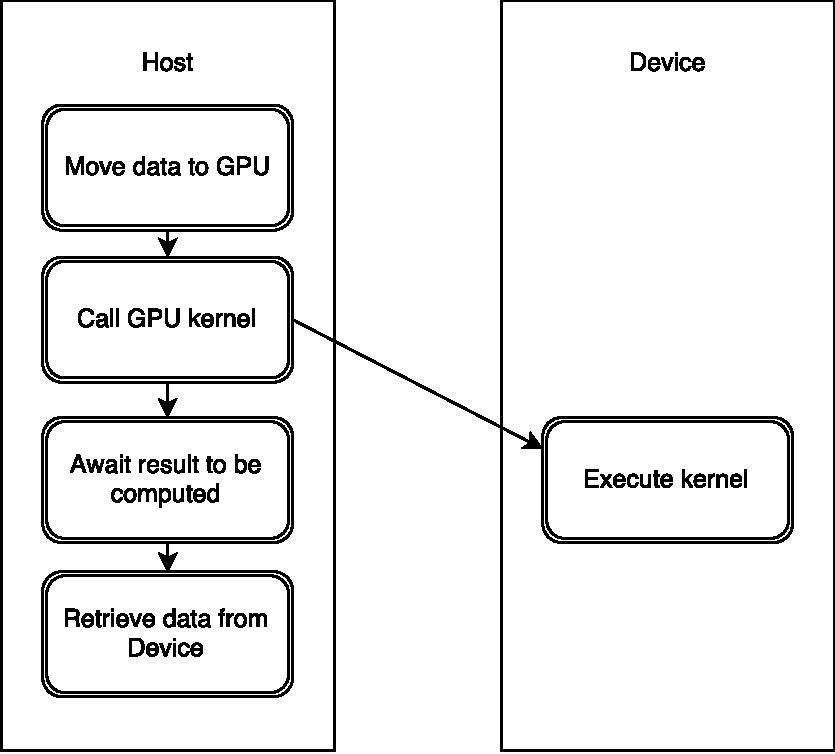
\includegraphics[scale=0.8]{figuras/cuda_execution_flow}
\caption{\label{fig:cuda_exec_flow}A typical CUDA execution flow.}
\end{figure}

CUDA kernels are organized into a set of blocks composed of a set of threads that cooperate 
with each other. The number of threads within a block and the number of blocks are specified 
at the launch moment, thus it can be adjusted to match the problem input size. The GPU's memory
hierarchy also reflects this organization \citep{kirk:2016}, since it is divided into four types: 
\begin{enumerate}
\item Registers: Private to each thread, it is used to hold frequently accessed data.

\item Shared Memory: It is a low latency memory shared between all threads within a block.

\item Constant Memory: A read-only memory that provides short latency and high bandwidth access.

\item Global Memory: A memory located outside the GPU processor chip. It can be accessed by all 
threads, but it is slower than all before-mentioned memories. It is the most abundant memory in 
the device. 
\end{enumerate}

\begin{figure}[htb]
\centering 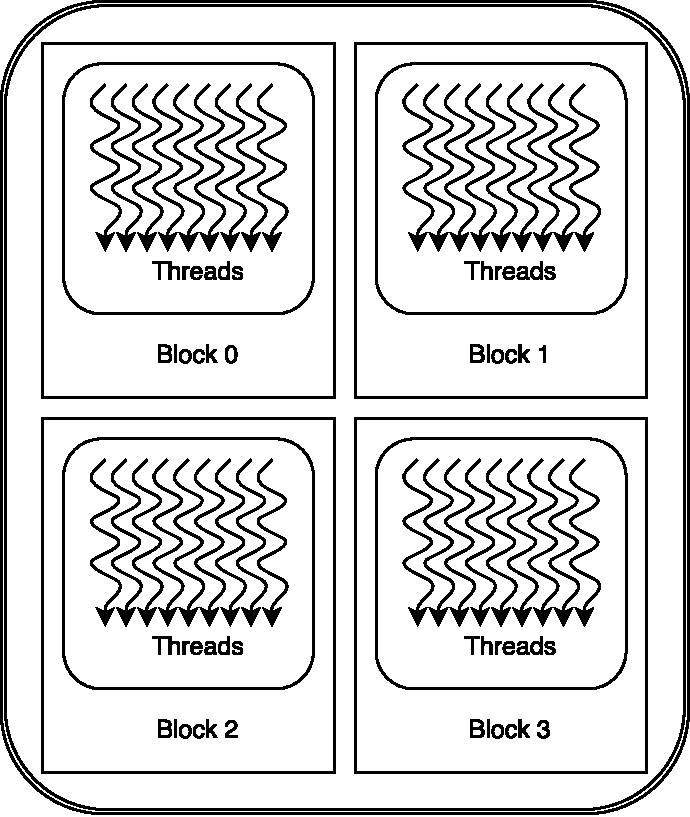
\includegraphics[scale=0.6]{figuras/threads_blocks}
\caption{\label{fig:cuda_exec_flow}Organization of a kernel execution with 9 threads per block and 4 blocks.}
\end{figure}

It must be highlighted that all threads may not run in parallel since it is limited to the amount of 
Streaming Multiprocessors (SM) the device has. Without entering in details, an SM is what schedules 
a set of 32 threads called Warps, executing each instruction in a SIMD fashion. Hence, the number of 
threads running in parallel is limited by the amount of SM available in the GPU. Because a GPU contains 
multiples SM, it is not considered a pure SIMD device.

In order to maximize the efficiency of a CUDA application, the programmer needs to minimize the memory 
transfer between CPU and GPU and explore any parallelism structure of the problem, as discussed in
\cite{devtalk_transfer:2012}.

\section {Related Works}

As GPUs became famous by its massively parallel capabilities and 
applications were developed to explore its potential, there is no 
surprise that researchers would use GPUs to accelerate
Boundary Elements Method implementations. 

\cite{torky:2017} presented an implementation for generating 
both $H$ and $G$ matrices of equation 1.2 with GPU acceleration 
using two CUDA kernels: One for computing the $G$ matrix and one 
for computing $H$ matrix. They also manage to keep the $H$ matrix 
in GPU memory to avoid host to device memory transfer to solve 
the linear system on the GPU, managing a 
108$\times$ speedup when building both $H$ and $G$ using single 
precision on a NVIDIA GeForce 770GTX when compared with an 
Intel Core i7-3770. For the linear system solving, the CPU required 
2.5h to complete, whereas with the GPU it would take 4s. This implies 
in a 2250 times speedup. As for precision, there is no further discussion 
rather than the usage of 10 points for the Gaussian Quadrature and that both 
CPU and GPU processed data in exactly the same manner and with reliable 
accuracy. 
